\ifdefined\inmaster\else\def\subonly{\jobname}\documentclass[12pt,oneside,openany]{book}
\usepackage{fullpage}
\makeatletter

%% Theorems
\usepackage{xcolor}
\definecolor{darkgreen}{rgb}{0,0.45,0} 
\usepackage[pagebackref,colorlinks,citecolor=darkgreen,linkcolor=darkgreen]{hyperref}
\usepackage{cleveref,aliascnt}
\def\defthm#1#2#3{%
  %% Ensure all theorem types are numbered with the same counter
  \newaliascnt{#1}{thm}
  \newtheorem{#1}[#1]{#2}
  \aliascntresetthe{#1}
  %% Tell cleveref's \cref what to call things
  \crefname{#1}{#2}{#3}}
\newtheorem{thm}{Theorem}[section]
\crefname{thm}{Theorem}{Theorems}
\theoremstyle{definition}
\defthm{defn}{Definition}{Definitions}
%\theoremstyle{remark}
\defthm{rmk}{Remark}{Remarks}
\defthm{advrmk}{Advanced Remark}{Advanced Remarks}
\newenvironment{adv}{\SMALL\begin{advrmk}}{\end{advrmk}}
\defthm{eg}{Example}{Examples}
\defthm{egs}{Examples}{Examples}

%% Reference format for sections
\crefformat{section}{\S#2#1#3}
\Crefformat{section}{Section~#2#1#3}
\crefrangeformat{section}{\S\S#3#1#4--#5#2#6}
\Crefrangeformat{section}{Sections~#3#1#4--#5#2#6}
\crefmultiformat{section}{\S\S#2#1#3}{ and~#2#1#3}{, #2#1#3}{ and~#2#1#3}
\Crefmultiformat{section}{Sections~#2#1#3}{ and~#2#1#3}{, #2#1#3}{ and~#2#1#3}
\crefrangemultiformat{section}{\S\S#3#1#4--#5#2#6}{ and~#3#1#4--#5#2#6}{, #3#1#4--#5#2#6}{ and~#3#1#4--#5#2#6}
\Crefrangemultiformat{section}{Sections~#3#1#4--#5#2#6}{ and~#3#1#4--#5#2#6}{, #3#1#4--#5#2#6}{ and~#3#1#4--#5#2#6}

%% Use the theorem counter for equations as well
\let\c@equation\c@thm
\numberwithin{equation}{section}

%% Pictures
\usepackage{tikz}

%% Differentials
\newcommand{\dd}{\ensuremath{\mathrm{d}}}
\newcommand{\dx}{\ensuremath{\dd x}}
\newcommand{\dy}{\ensuremath{\dd y}}
\newcommand{\dz}{\ensuremath{\dd z}}
\newcommand{\dt}{\ensuremath{\dd t}}
\newcommand{\du}{\ensuremath{\dd u}}
\newcommand{\dv}{\ensuremath{\dd v}}
\newcommand{\df}{\ensuremath{\dd f}}
\newcommand{\dg}{\ensuremath{\dd g}}
\newcommand{\dr}{\ensuremath{\dd r}}
\newcommand{\drho}{\ensuremath{\dd \rho}}
\newcommand{\dtheta}{\ensuremath{\dd \theta}}
\newcommand{\dphi}{\ensuremath{\dd \phi}}
\newcommand{\dpx}{\ensuremath{\dd \pt{x}}}

%% Partial derivatives
\newcommand{\pder}[2]{\frac{\partial #1}{\partial #2}}

%% Transposing vectors into forms
\newcommand{\tr}[1]{{#1}^\top}
\newcommand{\ptr}[1]{{(#1)}^\top}

%% Hodge star on forms
\newcommand{\str}[1]{{#1}^*}
\newcommand{\pstr}[1]{{(#1)}^*}

%% Points and vectors
\newcommand{\pt}[1]{\mathbf{#1}}
\newcommand{\ptc}[1]{(#1)}
\newcommand{\vc}[1]{\vec{#1}}
\newcommand{\vcc}[1]{(#1)}

%% Vector operations
\newcommand{\mgn}[1]{\Vert #1 \Vert}
\newcommand{\dotp}[2]{\langle #1 , #2 \rangle}
\newcommand{\crossp}[2]{#1 \times #2}

%% Fractions
\newcommand{\half}{\ensuremath{\textstyle\frac{1}{2}}}
\newcommand{\third}{\ensuremath{\textstyle\frac{1}{3}}}

%% Orders
\renewcommand{\th}{^{\mathrm{th}}}
\newcommand{\st}{^{\mathrm{st}}}

%% Approximation to specified order
\newcommand{\apx}[1]{\mathrel{\overset{#1}{\approx}}}

\makeatother


\usepackage{newclude}
\def\inmaster{1}
\ifdefined\subonly\includeonly{\subonly}\fi

\begin{document}

\documentclass[12pt]{amsart}
\usepackage{fullpage}
\makeatletter

%% Theorems
\usepackage{xcolor}
\definecolor{darkgreen}{rgb}{0,0.45,0} 
\usepackage[pagebackref,colorlinks,citecolor=darkgreen,linkcolor=darkgreen]{hyperref}
\usepackage{cleveref,aliascnt}
\def\defthm#1#2#3{%
  %% Ensure all theorem types are numbered with the same counter
  \newaliascnt{#1}{thm}
  \newtheorem{#1}[#1]{#2}
  \aliascntresetthe{#1}
  %% Tell cleveref's \cref what to call things
  \crefname{#1}{#2}{#3}}
\newtheorem{thm}{Theorem}[section]
\crefname{thm}{Theorem}{Theorems}
\theoremstyle{definition}
\defthm{defn}{Definition}{Definitions}
%\theoremstyle{remark}
\defthm{rmk}{Remark}{Remarks}
\defthm{advrmk}{Advanced Remark}{Advanced Remarks}
\newenvironment{adv}{\SMALL\begin{advrmk}}{\end{advrmk}}
\defthm{eg}{Example}{Examples}
\defthm{egs}{Examples}{Examples}

%% Reference format for sections
\crefformat{section}{\S#2#1#3}
\Crefformat{section}{Section~#2#1#3}
\crefrangeformat{section}{\S\S#3#1#4--#5#2#6}
\Crefrangeformat{section}{Sections~#3#1#4--#5#2#6}
\crefmultiformat{section}{\S\S#2#1#3}{ and~#2#1#3}{, #2#1#3}{ and~#2#1#3}
\Crefmultiformat{section}{Sections~#2#1#3}{ and~#2#1#3}{, #2#1#3}{ and~#2#1#3}
\crefrangemultiformat{section}{\S\S#3#1#4--#5#2#6}{ and~#3#1#4--#5#2#6}{, #3#1#4--#5#2#6}{ and~#3#1#4--#5#2#6}
\Crefrangemultiformat{section}{Sections~#3#1#4--#5#2#6}{ and~#3#1#4--#5#2#6}{, #3#1#4--#5#2#6}{ and~#3#1#4--#5#2#6}

%% Use the theorem counter for equations as well
\let\c@equation\c@thm
\numberwithin{equation}{section}

%% Pictures
\usepackage{tikz}

%% Differentials
\newcommand{\dd}{\ensuremath{\mathrm{d}}}
\newcommand{\dx}{\ensuremath{\dd x}}
\newcommand{\dy}{\ensuremath{\dd y}}
\newcommand{\dz}{\ensuremath{\dd z}}
\newcommand{\dt}{\ensuremath{\dd t}}
\newcommand{\du}{\ensuremath{\dd u}}
\newcommand{\dv}{\ensuremath{\dd v}}
\newcommand{\df}{\ensuremath{\dd f}}
\newcommand{\dg}{\ensuremath{\dd g}}
\newcommand{\dr}{\ensuremath{\dd r}}
\newcommand{\drho}{\ensuremath{\dd \rho}}
\newcommand{\dtheta}{\ensuremath{\dd \theta}}
\newcommand{\dphi}{\ensuremath{\dd \phi}}
\newcommand{\dpx}{\ensuremath{\dd \pt{x}}}

%% Partial derivatives
\newcommand{\pder}[2]{\frac{\partial #1}{\partial #2}}

%% Transposing vectors into forms
\newcommand{\tr}[1]{{#1}^\top}
\newcommand{\ptr}[1]{{(#1)}^\top}

%% Hodge star on forms
\newcommand{\str}[1]{{#1}^*}
\newcommand{\pstr}[1]{{(#1)}^*}

%% Points and vectors
\newcommand{\pt}[1]{\mathbf{#1}}
\newcommand{\ptc}[1]{(#1)}
\newcommand{\vc}[1]{\vec{#1}}
\newcommand{\vcc}[1]{(#1)}

%% Vector operations
\newcommand{\mgn}[1]{\Vert #1 \Vert}
\newcommand{\dotp}[2]{\langle #1 , #2 \rangle}
\newcommand{\crossp}[2]{#1 \times #2}

%% Fractions
\newcommand{\half}{\ensuremath{\textstyle\frac{1}{2}}}
\newcommand{\third}{\ensuremath{\textstyle\frac{1}{3}}}

%% Orders
\renewcommand{\th}{^{\mathrm{th}}}
\newcommand{\st}{^{\mathrm{st}}}

%% Approximation to specified order
\newcommand{\apx}[1]{\mathrel{\overset{#1}{\approx}}}

\makeatother

\title{On differential forms}
\begin{document}
\maketitle

In your previous calculus classes, you may or may not have encountered \emph{differential forms} by name.
However, you've certainly met them, even if you didn't realize it.
When you write
\[ \int_{x=a}^b f(x) \,\dx \]
the thing being integrated, ``$f(x) \,\dx$'', is a differential form.

You may have been told that the ``$\dx$'' is simply a notation that indicates which variable we're integrating, but this is a lie.
In multivariable calculus, we can no longer maintain this fiction: we have to treat differential forms as honest objects.
Fortunately, we also have two advantages over one-variable calculus in understanding differential forms: we have \emph{vectors} at our disposal; and some things are actually \emph{less} confusing in more dimensions because there are fewer coincidences to get confused by.

\section{Differential forms}
\label{sec:differential-forms}

If $\dx$ isn't just a notation indicating the integration variable, what is it?
If you encountered differentials in one-variable calculus, you may have been told that $\dx$ is a small change in $x$ (sometimes denoted $\Delta x$), or even an ``infinitesimal'' change in $x$.
These are not wrong, but with vectors we can give a better definition.

\begin{defn}
  A \textbf{differential form} is a function whose input is a point $\ptx$ \emph{and} a vector based at $\ptx$.
  We denote the vector by $\dpx$.
\end{defn}

In $n$ dimensions, the point $\ptx$ has $n$ coordinates, as does the vector $\dpx$.
As usual, in 2 or 3 dimensions we denote the coordinates of $\ptx$ by $\ptc{x,y}$ or $\ptc{x,y,z}$.
Similarly, we denote the coordinates of $\dpx$ by $\vcc{\dx,\dy}$ or $\vcc{\dx,\dy,\dz}$.
We can then describe a differential form by a formula involving these coordinates $x,y,z,\dx,\dy,\dz$.

We usually denote differential forms by lowercase Greek letters such as the following.
\begin{itemize}
\item $\omega$ (omega, not to be confused with the English letter $w$)
\item $\eta$ (eta, not to be confused with the English letter $n$)
\end{itemize}
Since a differential form $\omega$ is a function of a point and a vector, we would write $\omega(\ptx,\dpx)$ for the value of $\omega$ at a point $\ptx$ and a vector $\dpx$, or $\omega(x,y,\dx,\dy)$ if we want to emphasize all the coordinates.

\begin{egs}\label{egs:differential-forms}
  The following are all differential forms:
  \begin{gather*}
    x^2 \,\dx + 2xy \, \dy\\
    \half({x-z}) \,\dx - 4\, \dy + e^y \,\dz\\
    1 + \dx + \half \dx^2 + \third \dx^3\\
    \sin(x + \dx) - \sin(x)\\
    \sqrt{\dx^2+\dy^2}
  \end{gather*}
\end{egs}

Note that although $\dx$ is two letters, we regard it as one symbol standing for one variable.
In particular, an expression such as $\dx^2$ means $(\dx)^2$, not $\dd(x^2)$.
(We will give a different meaning to $\dd(x^2)$ in \cref{sec:differentials}.)

The first two of \cref{egs:differential-forms} are special in the following way.

\begin{defn}
  A \textbf{linear} differential form is one defined by an expression such as
  \[ f(\ptx) \, \dx + g(\ptx) \, \dy + h(\ptx) \, \dz. \]
  Here $f$, $g$, and $h$ are functions of the point $\ptx$ only, and each of them is multiplied by one of the coordinates of $\dpx$.
\end{defn}

Most mathematicians only use the term ``differential form'' for linear ones.
However, the more general ones are quite useful.

\begin{adv}
  To be more precise, the differential forms we are considering so far are \emph{1-cojet differential 1-forms}.
  Later on, we will encounter both $k$-cojet differential forms and differential $n$-forms for larger values of $k$ and $n$.
  However, until then, we will just use ``differential form'' for the notion defined above.
\end{adv}

It is helpful to think of the coordinates $\dx$, $\dy$, and $\dz$ as small changes in the values of the coordinates $x$, $y$, and $z$ respectively.
Here by \emph{small} we mean \emph{small relative to the values generally taken by $x$}.
For instance, if $x=3$, then a possible small change would be $\dx = 0.01$.
In this case, a differential form such as $\dx^2$ is an \emph{even smaller} change, since $\dx^2 = 0.0001$.

We say that $\dx$ is a \emph{first order} form while $\dx^2$ is \emph{second order}.
Similarly, we say that $x$ itself is \emph{zeroth order}, as is any function value $f(\ptx)$ not involving $\dpx$.

Every linear form is first-order: when we multiply a zeroth order form like $f(\ptx)$ by a first order one like $\dx$, the result is first order.
For instance, if $f(x) = 4$ and $\dx = 0.001$, then $f(x)\,\dx = 0.004$, which is about the same size as $\dx$.

The concept of order can be applied even to forms that are not polynomials in $\dx$.
For instance, if $\dx=0.01$, then $\sin(\dx) \approx 0.0099998$, which is about the same size as $\dx$.
Thus, it is reasonable to say that $\sin(\dx)$ is also first-order.
On the other hand, still with $\dx=0.01$, we have $\cos(\dx) - 1 \approx -0.00005$, which is much smaller than $\dx$ and about the same size as $\dx^2$.
Thus, it is reasonable to say that $\cos(\dx) - 1$ is second-order.

We will not make precise the general notion of ``order''; it can be done, but it is a bit complicated and not necessary for our purposes.
(If you're curious, see the optional handout.)
All that we will need is a definition of when a differential form is \emph{smaller than first order} (e.g.\ second-order or third-order).
This is because in calculus, we are concerned with \emph{approximations to first order}, also known as \emph{linear approximations}; and forms that are smaller than first order do not affect these approximations.
Thus, we will call them \emph{negligible} (to first order).

\begin{defn}\label{def:negligible}
  A differential form $\omega$ is called \textbf{negligible} at a point $\ptx$ if
  \[ \lim_{\dpx\to\vc{0}} \frac{\omega(\ptx,\dpx)}{\mgn{\dpx}} = 0. \]
\end{defn}

Recall that definitions in mathematics introduce a \emph{new} meaning for a word.
Thus, \emph{from now on} (in this class) the word ``negligible'' \emph{will mean} what this definition says it does.
Our previous discussion was only motivational; the definition is the ``gold standard'' for the meaning of the word.

The first thing to do in understanding a definition is to look at some examples.
If we chose the definition well, the examples will justify our motivation.

\begin{eg}
  The differential form $\dx^2$ is negligible at any point.
  To see this, note that
  \[ \frac{\dx^2}{\mgn{\dpx}} = \frac{\dx}{\mgn{\dpx}} \,\dx \]
  and $\frac{\dx}{\mgn{\dpx}}\le 1$ everywhere, while $\lim_{\dpx\to\vc{0}} \dx = 0$.
  Thus, the limit of their product is also $0$.
  Similarly, the following differential forms are all negligible:
  \[ \dy^2 \qquad \dx\,\dy \qquad \dx^3 \qquad \dx\,\dy^2\,\dz \]
\end{eg}

\begin{eg}
  By a similar argument, if $\omega$ is bounded for values of $\dpx$ near $\vc{0}$, while $\eta$ is negligible at $\ptx$, then their product $\omega\eta$ is also negligible at $\ptx$.
  In particular, this is true if $\omega$ is a function of $\ptx$ only, at any point where it is defined.
  For instance, the following differential forms are negligible:
  \begin{gather*}
    x^2\,\dx\,\dy\\
    e^{-x^2+y^2} \,\dy^2
  \end{gather*}
\end{eg}

\begin{eg}
  If $\omega$ and $\eta$ are negligible at $\ptx$, then so is their sum $\omega+\eta$, by the sum rule for limits.
  Thus, the following differential forms are negligible:
  \begin{gather*}
    \dx^2 + \dy^2\\
    x^2 \,\dx\,\dy + e^{y}\,\dy\,\dz^2
  \end{gather*}
\end{eg}

Notice that all the examples of negligible forms are what we would intuitively call second-order or higher.
We will continue to use the informal terminology of ``first-order'', ``second-order'', and so on when discussing forms.
However, in definitions and theorems we will use only the term ``negligible'' that we have defined precisely.


\section{Graphing differential forms}
\label{sec:graphing-differential-forms}

A differential form should be thought of as giving for each point $\ptx$, a function of the vector $\dpx$, which represents the ``displacement from $\ptx$'' of another point (namely, the point $\ptx+\dpx$).
In addition, we generally only care about this function for small values of $\dpx$.

We can give an idea of what such a thing looks like by drawing at each point $\ptx$ a small fragment of the graph of the corresponding function of $\dpx$, with its origin placed at $\ptx$.
This is easiest to do in one dimension.
For instance, we would graph the form $x\,\dx$ as follows.
\begin{center}
  \begin{tikzpicture}
    \draw[<->] (-5,0) -- (5,0);
    \draw[<->] (0,-2) -- (0,2);
    \draw (2,.2) -- (2,-.2) node[below right] {$1$};
    \draw (4,.2) -- (4,-.2) node[below right] {$2$};
    \draw (-2,.2) -- (-2,-.2) node[below] {$-1$};
    \draw (-4,.2) -- (-4,-.2) node[below left] {$-2$};
    \begin{scope}[blue,very thick]
      \draw (-.3,0) -- (.3,0);
      \draw (.7,-.15) -- (1.3,.15);
      \draw (1.7,-.3) -- (2.3,.3);
      \draw (2.7,-.45) -- (3.3,.45);
      \draw (3.7,-.6) -- (4.3,.6);
      \draw (-.7,-.15) -- (-1.3,.15);
      \draw (-1.7,-.3) -- (-2.3,.3);
      \draw (-2.7,-.45) -- (-3.3,.45);
      \draw (-3.7,-.6) -- (-4.3,.6);
    \end{scope}
  \end{tikzpicture}
\end{center}
Here at the point $(1,0)$ we have graphed a piece of the function $f(\dx) = \dx$, with its origin at $(1,0)$.
Similarly, at $(2,0)$ we have graphed a piece of $f(\dx) = 2\,\dx$, with its origin at $(2,0)$, and so on.

Analogously, we would graph $x\,\dx^2$ as follows, drawing $f(\dx) = \dx^2$ with origin at $(1,0)$, and $f(\dx)=2\,\dx^2$ with origin at $(2,0)$, etc.
\begin{center}
  \begin{tikzpicture}
    \draw[<->] (-5,0) -- (5,0);
    \draw[<->] (0,-2) -- (0,2);
    \draw (2,.2) -- (2,-.2) node[below right] {$1$};
    \draw (4,.2) -- (4,-.2) node[below right] {$2$};
    \draw (-2,-.2) -- (-2,.2) node[above] {$-1$};
    \draw (-4,-.2) -- (-4,.2) node[above] {$-2$};
    \begin{scope}[blue,very thick]
      \draw (-.3,0) -- (.3,0);
      % \draw (.7,-.15) -- (1.3,.15);
      \draw (1.7,.3) to[out=-60,in=180] (2,0) to[out=0,in=-120] (2.3,.3);
      % \draw (2.7,-.45) -- (3.3,.45);
      \draw (3.7,.6) to[out=-75,in=180,looseness=.5] (4,0) to[out=0,in=-105,looseness=.5] (4.3,.6);
      % \draw (-.7,-.15) -- (-1.3,.15);
      \draw (-1.7,-.3) to[out=120,in=0] (-2,0) to[out=180,in=60] (-2.3,-.3);
      % \draw (-2.7,-.45) -- (-3.3,.45);
      \draw (-3.7,-.6) to[out=105,in=0,looseness=.5] (-4,0) to[out=180,in=75,looseness=.5] (-4.3,-.6);
    \end{scope}
  \end{tikzpicture}
\end{center}
In the previous two examples, all the small graphs lay along the $x$-axis, because the differential forms being graphed had no zeroth order term.
If there is a zeroth order term, then the small graphs will lie along the graph of that term.
For instance, here is a graph of $-x^2 + \sin(x)\,\dx$, with the curve $y=-x^2$ shown as well for comparison:
\begin{center}
  \begin{tikzpicture}
    \draw[<->] (-5,0) -- (5,0);
    \draw[<->] (0,-5) -- (0,1);
    \draw (2,-.2) -- (2,.2) node[above] {$\frac\pi2$};
    \draw (4,-.2) -- (4,.2) node[above] {$\pi$};
    \draw (-2,-.2) -- (-2,.2) node[above] {$-\frac\pi2$};
    \draw (-4,-.2) -- (-4,.2) node[above] {$-\pi$};
    \draw (.2,-1) -- (-.2,-1) node[left] {$-\frac{\pi^2}{4}$};
    \draw (.2,-4) -- (-.2,-4) node[left] {$-\pi^2$};
    \begin{scope}[blue,very thick]
      \draw (-.3,0) -- (.3,0);
      \draw (.7,-.4) -- (1.3,-.1);
      \draw (1.7,-1.3) -- (2.3,-.7);
      \draw (2.7,-2.65) -- (3.3,-2.35);
      \draw (3.7,-4) -- (4.3,-4);
      \draw (-.7,-.4) -- (-1.3,-.1);
      \draw (-1.7,-1.3) -- (-2.3,-.7);
      \draw (-2.7,-2.65) -- (-3.3,-2.35);
      \draw (-3.7,-4) -- (-4.3,-4);
    \end{scope}
    \draw[purple,dashed] (-4,-4) to[out=60,in=120,looseness=1.97] (4,-4);
  \end{tikzpicture}
\end{center}

We can also draw differential forms in multiple variables, although it is rather trickier.\dots
% TODO: Do that.

We now consider some differential forms of particular interest associated to a function $f$ of $x$.
As a running example we will consider the following function:
\def\axes{
    \draw[<->] (-5,0) -- (5,0);
    \draw[<->] (0,-2) -- (0,2);
    \foreach \x in {1,2,3,4} \draw (\x,.2) -- (\x,-.2);
    \foreach \x in {1,2,3,4} \draw (-\x,.2) -- (-\x,-.2);
}
\def\fctn#1{\draw[#1] (-5,.3) to[out=30,in=170] (-4,1) to[out=-10,in=110] (-2,-1.2) to[out=-70,in=-130] (1,.2) to[out=50,in=120] (5,-.5);}
\def\heights{-4/1cm/-.05,-3/.55cm/-.3,-2/-1.2cm/-.6,-1/-1.5cm/.15,0/-.85cm/.28,1/.2cm/.32,2/.81cm/.08,3/.85cm/-.05,4/.47cm/-.18}
\begin{center}
  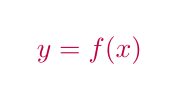
\begin{tikzpicture}
    \axes
    \fctn{purple,very thick}
    \node[purple,below right] at (5,-.5) {$y=f(x)$};
  \end{tikzpicture}
\end{center}
First of all, we can regard $f(x)$ itself as a differential form: one which simply does not use the variable $\dx$ (and thus takes the same value regardless of what $\dx$ is).
Thus, each little piece of the graph of this differential form will be a horizontal line, as shown below (we have included the graph of $f$ for comparison).
\begin{center}
  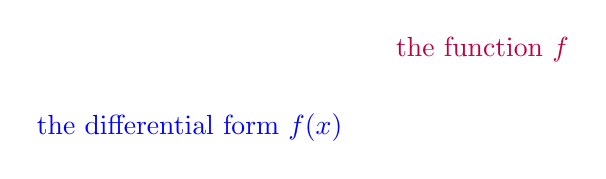
\begin{tikzpicture}
    \axes
    \fctn{dashed,purple}
    \node[purple,right] at (5,-.5) {the function $f$};
    \foreach \x/\y in \heights \draw[blue,very thick] (\x-.3,\y) -- (\x+.3,\y);
    \node[blue] at (2.5,-1.5) {the differential form $f(x)$};
  \end{tikzpicture}
\end{center}
This seems a little odd as a representation of $f$, so we may ask whether there is some differential form for which each piece of its graph looks like a corresponding part of the graph of $f$ itself.
Such a differential form is $f(x+\dx)$, since as $\dx$ varies around zero, $x+\dx$ varies around $x$.
\begin{center}
  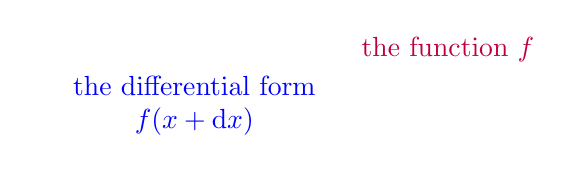
\begin{tikzpicture}
    \axes
    \fctn{dashed,purple}
    \node[purple,below right] at (5,-.5) {the function $f$};
    \foreach \x/\y in \heights {
      \begin{scope}
        \clip (\x-0.3,\y-0.3cm) rectangle (\x+0.3,\y+0.3cm);
        \fctn{blue,very thick}
      \end{scope}
    }
    \node[blue] at (3,-1.5) {\parbox{4cm}{\centering the differential form\\$f(x+\dx)$}};
  \end{tikzpicture}
\end{center}
Finally, consider the differential form $f(x+\dx)-f(x)$.
Its graph at $x$ looks just like a piece of the graph of $f$ near $x$, just as for the form $f(x+\dx)$, but now this graph is shifted down so that it crosses the $x$-axis at the point $(x,0)$ (this is what subtracting $f(x)$ accomplishes).
\begin{center}
  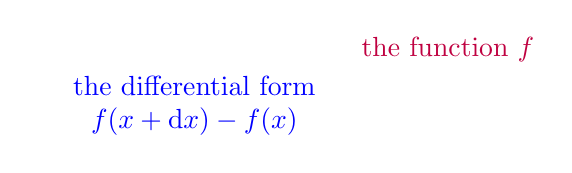
\begin{tikzpicture}
    \axes
    \fctn{dashed,purple}
    \node[purple,below right] at (5,-.5) {the function $f$};
    \foreach \x/\y in \heights {
      \begin{scope}
        \clip (\x-.3,-.3) rectangle (\x+0.3,.3);
        \fctn{blue,very thick,yshift=-\y}
      \end{scope}
    }
    \node[blue] at (3,-1.5) {\parbox{4cm}{\centering the differential form\\$f(x+\dx)-f(x)$}};
  \end{tikzpicture}
\end{center}
Note that the pieces of the graph of $f(x+\dx)-f(x)$ all look quite close to straight lines.
This happens whenever we ``zoom in'' sufficiently on a smooth function, and it is this observation that leads to the idea of differentiation.


\section{Differentials}
\label{sec:differentials}

In one-variable calculus, you may have encountered the differential of a function.
Namely, if $f$ is a function of one variable $x$, then its differential is
\begin{equation}
  \df = f'(x) \, \dx\label{eq:onevariable-differential}
\end{equation}
where $f'$ is the \emph{derivative} of $f$.
Note that $\df$ is a differential form.
Its graph looks like this (the function $f$ is the same one we were using as an example at the end of the last section).
\begin{center}
  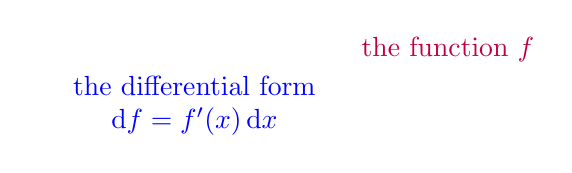
\begin{tikzpicture}
    \axes
    \fctn{dashed,purple}
    \node[purple,below right] at (5,-.5) {the function $f$};
    \foreach \x/\y/\slope in \heights {
      \begin{scope}
        \clip (\x-.3,-.3) rectangle (\x+0.3,.3);
        % \fctn{red,very thick,yshift=-\y}
        \draw[blue,very thick] (\x-.3,-\slope) -- (\x+.3,\slope);
      \end{scope}
    }
    \node[blue] at (3,-1.5) {\parbox{4cm}{\centering the differential form\\$\df = f'(x) \,\dx$}};
  \end{tikzpicture}
\end{center}
Note that this is barely distinguishable from the graph of $f(x+\dx)-f(x)$.
This is the whole point of the derivative: $f'(x)$ is the slope of the tangent line to the graph of $f$ at $x$, and that line is the best possible \emph{linear approximation} to the graph.
Indeed, recall that by definition, the derivative is
\[ f'(x) = \lim_{\dx\to 0} \frac{f(x+\dx)-f(x)}{\dx} \]
Thus, when $\dx$ is small, we can say that
\begin{equation}\label{eq:difference-quotient-close-derivative}
  \frac{f(x+\dx)-f(x)}{\dx}\quad\text{is very close to}\quad f'(x).
\end{equation}
Multiplying each of these by $\dx$, we find that
\begin{equation}
  f(x+\dx)-f(x) \quad\text{is very close to}\quad f'(x)\,\dx.\label{eq:difference-close-differential}
\end{equation}
This is what we saw in the above-remarked similarity of graphs.

\begin{adv}
  However, the quantities in~\cref{eq:difference-close-differential} are of a different order than those in~\cref{eq:difference-quotient-close-derivative}:
  $\frac{f(x+\dx)-f(x)}{\dx}$ and $f'(x)$ are zeroth order, while $f(x+\dx)-f(x)$ and $f'(x)\,\dx$ are first order.
  Thus, the precise meaning of ``close'' is different: in~\cref{eq:difference-close-differential} we mean that their difference is first order, while in~\cref{eq:difference-quotient-close-derivative} we mean that their difference is second order.
  This is why \cref{def:differential} below is phrased as it is.
\end{adv}

\Cref{eq:onevariable-differential} from one-variable calculus defines the \emph{differential} of $f$ in terms of the \emph{derivative} of $f$.
However, in multivariable calculus, it is more appropriate to do things in the other order, using the idea of~\cref{eq:difference-quotient-close-derivative} to define the differential \emph{first}, and then deducing a notion of ``derivative'' from this.

\begin{defn}\label{def:differential}
  If $f$ is a function of a point $\ptx$, then its \textbf{differential} is a linear differential form $\df$ such that
  \[ f(\ptx + \dd\ptx) - f(\ptx) - \df \]
  is negligible at $\ptx$.
  If such a form $\df$ exists, we say that $f$ is \textbf{differentiable} at $\ptx$.
\end{defn}

As always, we should explore a new definition with examples.

\begin{eg}
  Let $f(x) = x^2$, an ordinary one-variable function.
  Then
  \begin{align*}
    f(x + \dx) - f(x) &= (x+\dx)^2 - x^2\\
    &= x^2 + 2 x \, \dx + \dx^2 - x^2\\
    &= 2x \, \dx + \dx ^2.
  \end{align*}
  What linear form $\dd f$ can we subtract from this to make it second order?
  We may think of subtracting $2x \, \dx$, leaving the second-order term $\dx^2$:
  \[ f(x + \dx) - f(x) - 2x \, \dx \;=\; \dx^2. \]
  Thus, we have $\dd(x^2) = 2 x \, \dx$.
  Of course, this is the same result that we would have gotten from \cref{eq:onevariable-differential}.
\end{eg}

\begin{eg}
  Let $f(x,y) = x^2 + 2y^2 - xy$.
  Then
  \begin{align*}
    f(x+\dx,y+\dy) - f(x,y)
    &= (x+\dx)^2 + 2(y+\dy)^2 - (x+\dx)(y+\dy) - x^2 - 2y^2 + xy\\
    &= x^2 + 2 x \, \dx + \dx^2 + 2y^2 + 4y\,\dy + 2\dy^2\\
    & \hspace{2cm} - x^2 - x \, \dy - y \, dx - \dx\, \dy - x^2 - 2y^2 + xy\\
    &= 2x\,\dx + 4y\,\dy - x\,\dy - y\,\dx + \dx^2 + 2\dy^2 - \dx\,\dy\\
    &= (2x-y)\,\,dx + (4y-x)\,\dy + (\dx^2 + 2\dy^2 - \dx\,\dy)
  \end{align*}
  In the last line we have separated this into a linear form plus one of second order.
  Thus, we have
  \[ \dd(x^2 + 2y^2 - xy) = (2x-y)\,\dx + (4y-x)\,\dy .\]
\end{eg}

\begin{eg}
  Consider $f(x) = \sin x$.
  Using the sum identity for sine, we have
  \begin{align}
    \sin(x+\dx) - \sin (x)
    &= \sin x \cos \dx + \sin \dx \cos x - \sin x \notag\\
    &= \cos x \sin \dx + (\sin x) (\cos \dx - 1).\label{eq:sine-difference}
  \end{align}
  The usual way to proceed from here is to recall the limits
  \[ \lim_{h\to 0} \frac{\sin h}{h} = 1 \qquad\text{and}\qquad
  \lim_{h\to 0} \frac{\cos h - 1}{h} = 0 \]
  The second says exactly that the form $\cos \dx - 1$ is negligible.
  The first one implies that
  \[ \lim_{\dx\to 0} \frac{\sin \dx - \dx}{\dx} = 0 \]
  and therefore the form $\sin \dx - \dx$ is negligible.
  Multiplying by the ordinary functions $\cos x$ and $\sin x$ doesn't change the order, so we can write
  \begin{align*}
    \sin(x+\dx) - \sin (x)
    &= \cos x \sin \dx + (\sin x) (\cos \dx - 1)\\
    &= (\cos x )(\dx  + \sin \dx - \dx) + (\sin x) (\cos \dx - 1)\\
    &= \cos x \,\dx + (\cos x) (\sin \dx - \dx) + (\sin x) (\cos \dx - 1)
  \end{align*}
  which is written as the linear form $\cos x \,\dx$ plus a negligible one.
  Thus, $\dd(\sin x) = \cos x \,\dx$.

  Another, perhaps more intuitive, way to proceed from \cref{eq:sine-difference} is to recall the power series expansions
  \begin{align*}
    \sin x &= x - \frac{x^3}{3!} + \frac{x^5}{5!} - \cdots\\[2pt]
    \cos x &= 1 - \frac{x^2}{2!} + \frac{x^4}{4!} - \cdots
  \end{align*}
  Therefore, we have
  \begin{align*}
    \sin \dx - \dx &= - \frac{\dx^3}{3!} + \frac{\dx^5}{5!} - \cdots\\[2pt]
    \cos \dx - 1 &= - \frac{\dx^2}{2!} + \frac{\dx^4}{4!} - \cdots.
  \end{align*}
  Using general facts about functions defined by power series, one can conclude from this that the first is third order and the second is second order; thus both are negligible.
  (However, when calculating the power series expansions of sine and cosine in one-variable calculus, you probably used the fact that you already knew their derivatives, so this would technically be a circular argument.)
\end{eg}

A convenient way to work with differentials is to introduce the notion of ``approximation to first order''.

\begin{defn}
  We say that two differential forms $\omega$ and $\eta$ are \textbf{equal to first order} if their difference $\omega-\eta$ is negligible.
  In this case we write
  \[\omega\apx1 \eta.\]
\end{defn}

\begin{eg}
  We have $x\,\dx + \dx^2 \apx1 x\,\dx - e^x \,\dx^2$, since their difference is
  \[ (x\,\dx + \dx^2) - (x\,\dx - e^x\, \dx^2) = (1+e^x)\dx^2 \]
  which is second order.
\end{eg}

The relation $\apx{1}$ behaves roughly like equality.
For instance, we can add or subtract the same differential form from both sides.
In particular, if $\omega$ is negligible, then $\omega\apx{1}0$, so we have $\eta + \omega \apx{1} \eta$ for any $\eta$.

\begin{eg}
  Since $4\,\dx^2$ is second order, we have $\sin(x) \,\dx + 4\, \dx^2 \apx{1} \sin(X)\,\dx$.
\end{eg}

We can also multiply both sides by any differential form that is bounded near $\dx=0$, since multiplying by such a form doesn't affect negligibility.

\begin{eg}
  Since $\sqrt{x}\, \dx^2$ is second order, we have
  \[x\,\dx \apx{1} x\,\dx + \sqrt{x}\, \dx^2\]
  Thus, we can multiply by $e^x$ to get
  \[x e^x \,\dx \apx{1} x e^x\,\dx + \sqrt{x}\, e^x\, \dx^2,\]
  or multiply by $\dx$ to get
  \[x\,\dx^2 \apx{1} x\,\dx^2 + \sqrt{x} \,\dx^3. \]
  The latter is fairly trivial, though since both sides are $\apx{1} 0$.
\end{eg}

Now we can equivalently state the definition of a differential: $\df$ is a linear differential form such that
\[ f(x+\dx) \apx1 f(x) + \df, \]
if such exists.
Our previous calculations of differentials can all be written in this way.
For instance,
\begin{align*}
  (x+\dx)^2 &= x^2 + 2 x\,\dx + \dx^2\\
  &\apx1 x^2 + 2 x\,\dx
\end{align*}
since $\dx^2$ is second order.
Therefore, $\dd(x^2) = 2x\,\dx$.

% TODO: Tangent planes and linear approximations

\section{Differential rules}
\label{sec:differential-rules}

We easily deduce all the usual derivative rules, written in terms of differentials.
For instance, given functions $f$ and $g$, consider their sum $f+g$.
\begin{align*}
  f(x+\dx) + g(x+\dx)
  &\apx1 f(x) + \df + g(x) + \dg\\
  &= \big[f(x) + g(x)\big] + \big[ \df + \df \big]
\end{align*}
Thus, we have
\[ \dd(f+g) = \df + \dg. \]

Similarly, for the product rule, we compute
\begin{align*}
  f(x+\dx) \, g(x+\dx)
  &\apx1 \big(f(x)+\df\big)\big(g(x) + \dg \big)\\
  &= f(x) g(x) + f(x) \,\dg + g(x) \,\df + \df\,\dg\\
  &\apx1 f(x) g(x) + f(x) \,\dg + g(x) \,\df
\end{align*}
since $\df\,\dg$ is a product of two first-order forms, hence second order.
Thus,
\[ \dd(f\,g) = f\,\dg + g\,\df.\]

Importantly, these rules, stated in exactly the same way, apply to functions of more than one variable.
\begin{eg}\label{eg:twovar-differential}
  If $f(x,y) = x^2y + xy^2$, then we can use the sum and product rules to obtain
  \begin{align*}
    \dd(x^2y + xy^2) &= \dd(x^2y) + \dd(xy^2)\\
    &= x^2\,\dy + y \,\dd(x^2) + x \,\dd(y^2) + y^2\,\dx\\
    &= x^2\,\dy + y \,(2x\,\dx) + x\, (2y\,\dy) + y^2\,\dx\\
    &= (2xy + y^2)\,\dx + (x^2+2xy)\,\dy
  \end{align*}
\end{eg}

Finally, the chain rule for differentials is easy to \emph{use}, but tricky to \emph{state}, because the notation makes it look like a triviality.
Suppose that we have a function $f$ of two variables $u$ and $v$, and that $u$ and $v$ are each themselves functions of two other variables $x$ and $y$.
Then the statement of the chain rule is that if we calculate $\df$ treating $u$ and $v$ as its input variables (obtaining a linear differential form involving $\du$ and $\dv$), and likewise we calculate the differentials $\du$ and $\dv$ treating $x$ and $y$ as their input variables (obtaining linear differential forms involving $\dx$ and $\dy$), then substitute the latter into the former, as well as the values of $u$ and $v$ in terms of $x$ and $y$, we obtain the same expression for $\df$ in terms of $\dx$ and $\dy$ that we would have if we first substituted the functions $u$ and $v$ and then took the differential treating $x$ and $y$ as the input variables.
If this was incomprehensible, you're in good company; it is much better explained by an example.

\begin{eg}
  Let $f(u,v) = u v + 3u$, while $u(x,y) = x-5y$ and $v(x,y) = 4y-x$.
  Then
  \begin{align*}
    \df &= \dd(u v) + \dd(3u)\\
    &= v \,\du + u\,\dv + 3 \,\du\\
    &= (v+3)\,\du + u\,\dv
  \end{align*}
  and
  \begin{align*}
    \du &= \dx - 5\, \dy\\
    \dv &= 4\,\dy - \dx
  \end{align*}
  Therefore,
  \begin{align*}
    \df &= (v+3)\,\du + u\,\dv\\
    &= (4y-x+3)\,(\dx - 5 \dy) + (x-5y) (4\,\dy - \dx) \\
    &= (9y-2x+3)\,\dx + (9x - 40y - 15)\,\dy.
  \end{align*}
  On the other hand, if we substituted first, we would have
  \begin{align*}
    f(u(x,y),v(x,y)) &= (x-5y)(4y-x) + 3(x-5y)\\
    &= 4xy - x^2 - 20y^2 + 5xy + 3x - 15 y\\
    &= 9xy - x^2 - 20y^2 + 3x - 15 y
  \end{align*}
  and therefore
  \begin{align*}
    \df &= 9x\, \dy + 9y\, \dx - 2 x\,\dx - 40 y\,\dy + 3\,\dx - 15\,\dy\\
    &= (9y - 2x +3)\,\dx + (9x - 40y - 15)\,\dy
  \end{align*}
  which is the same result.
\end{eg}

When expressed in terms of differentials in this way, the chain rule is also known as \emph{Cauchy's invariant rule}.
Of course, it is mainly useful in cases where we are given the result of substitution, but where it is not obvious how to find the differential until we decompose it.

\begin{eg}
  Consider the function $f(x,y) = \sin (xy)$.
  We can find the differential by letting $u=xy$; then we have $f = \sin(u)$, and hence
  \begin{align*}
    \df &= \cos(u)\,\du\\
    \du &= x\,\dy + y\,\dx
  \end{align*}
  and therefore
  \begin{align*}
    \df &= \cos(u)\,\du \\
    &= \cos(xy) (x\,\dy + y\,\dx)\\
    &= y\cos(xy)\,\dx + x\cos(xy)\,\dy
  \end{align*}
  Once we are more familiar with the operation of the chain rule, this calculation can be done without naming the variable $u$.
  We simply remember that in the rule for the derivative of the sine function, $\dd(\sin(x)) = \cos(x) \, \dx$, the variable $x$ can be replaced by \emph{any expression}, as long as we also remember to replace $\dx$ by the differential of \emph{that expression}.
  \begin{align*}
    \df &= \dd(\sin(xy))\\
    &= \cos(xy) \, \dd(xy)\\
    &= \cos(xy) (x\,\dy + y\,\dx)\\
    &= y\cos(xy)\,\dx + x\cos(xy)\,\dy.
  \end{align*}
\end{eg}

The proof of the chain rule is somewhat tricky; we omit it.
\begin{notextbook}(It might be given in your textbook.)\end{notextbook}

A particularly important example of the chain rule is translating between different coordinate systems.
Recall that in addition to the usual ``rectangular'' or ``Cartesian'' coordinates $x$ and $y$ on the plane, we can use \emph{polar coordinates} $r$ and $\theta$, which are related by the equations
\begin{alignat*}{2}
  x &= r \cos \theta &\qquad r &= \sqrt{x^2+y^2}\\
  y &= r \sin\theta &\qquad \tan \theta &= y/x
\end{alignat*}
(It would not be correct to write ``$\theta = \arctan(y/x)$'', since $\arctan$ only takes values between $-\pi/2$ and $\pi/2$, whereas $\theta$ usually ranges from $0$ to $2\pi$.)
Differentiating these equations, we obtain corresponding equations relating the differentials of these variables.
\begin{align}
  \dx &= \cos \theta \,\dr - r \sin\theta \,\dtheta \label{eq:polar-dx} \\
  \dy &= \sin\theta \,\dr + r \cos\theta\,\dtheta \label{eq:polar-dy}\\
  \dr &= \frac{1}{2\sqrt{x^2+y^2}}(2x\,\dx + 2y\,\dy) \notag\\
  &= \frac{x}{\sqrt{x^2+y^2}}\,\dx + \frac{y}{\sqrt{x^2+y^2}}\,\dy
  \qquad\left(= \frac{x}{r} \,\dx + \frac{y}{r}\,\dy\right) \notag\\
  \frac{1}{(\cos \theta)^2} \,\dtheta &= \frac{1}{x}\,\dy - \frac{y}{x^2}\,\dx \notag\\
  \dtheta &= (\cos \theta)^2 \left( \frac{r}{r^2\cos\theta}\,\dy - \frac{y}{r^2 (\cos\theta)^2}\,\dx\right) \notag\\
  &= \frac{x}{r^2} \,\dy - \frac{y}{r^2} \,\dx \notag\\
  &= \frac{x}{x^2+y^2} \,\dy - \frac{y}{x^2+y^2} \,\dx \notag
\end{align}
(We could also obtain the same equations for $\dr$ and $\dtheta$ by solving for them in the first two equations.)
It follows that if $f$ is written as a function of $x$ and $y$, we can find its differential with respect to $r$ and $\theta$ by substituting these relations into its differential with respect to $x$ and $y$, and vice versa.

\begin{eg}
  Suppose $f(x,y) = e^{x^2+y^2}$.
  Then we have
  \begin{align*}
    \df &= e^{x^2+y^2} (2x \,\dx + 2y\,\dy)\\
    &= 2x e^{x^2+y^2} \,\dx + 2y e^{x^2+y^2} \,\dy\\
    &= 2 r\cos\theta e^{r^2} \, (\cos \theta \,\dr - r \sin\theta \,\dtheta) + 2r\sin\theta e^{r^2} (\sin\theta \,\dr + r \cos\theta\,\dtheta)\\
    &= 2r e^{r^2} ((\cos\theta)^2 + (\sin\theta)^2)\,\dr + 2r^2 e^{r^2}(\sin\theta\cos\theta - \cos\theta\sin\theta) \dtheta\\
    &= 2r e^{r^2}\,\dr.
  \end{align*}
  which is the same result that we could calculate directly by writing $f = e^{r^2}$ and thus
  \begin{align*}
    \df &= e^{r^2} \, (2r\,\dr).
  \end{align*}
\end{eg}

Similarly, in three-dimensional space, in addition to the rectangular coordinates $x$, $y$, and $z$, we have both \emph{cylindrical} coordinates $r$, $\theta$, and $z$, and \emph{spherical} coordinates $\rho$, $\theta$, and $\phi$.
Cylindrical coordinates are related to rectangular ones in three dimensions in the same way that polar coordinates are related to rectangular ones in two dimensions, with $z$ coming along untouched for the ride.
For spherical coordinates we have
\begin{align*}
  x &= \rho \cos\theta \sin\phi\\
  y &= \rho \sin\theta \sin\phi\\
  z &= \rho\cos\phi
\end{align*}
and hence
\begin{align*}
  \dx &= \cos\theta \sin\phi \,\drho - \rho\sin\theta\sin\phi \,\dtheta + \rho\cos\theta\cos\phi \,\dphi\\
  \dy &= \sin\theta \sin\phi\,\drho + \rho\cos\theta\sin\phi \,\dtheta + \rho\sin\theta\cos\phi \,\dphi\\
  \dz &= \cos\phi\,\drho - \rho\sin\phi\,\dphi
\end{align*}
We leave it to the reader to write out the reverse expressions for spherical coordinates in terms of rectangular ones.


\section{Derivatives}
\label{sec:derivatives}

We can now define the \emph{derivative} in terms of the \emph{differential}.
Note that in one dimension, a linear differential form must be of the form
\[ g(x) \,\dx \]
for some function $g$.
In particular, if $f$ is a differentiable function of one variable $x$, then $\df = g(x) \, \dx$ for some function $g$, which we call the \emph{derivative} of $f$ and denote by $f'$.
In other words, $\df = f'(x)\,\dx$ (this is \cref{eq:onevariable-differential}), or
\[ f'(x) = \frac{\df}{\dx}. \]
This is a notation that you have probably seen before.
The point is that now, we have given separate meanings to $\dx$ and $\df$, and \emph{defined} $f'(x)$ to be their quotient.

However, when there is more than one variable, this doesn't work any more!
For instance, consider the function $f(x,y) = x^2y + xy^2$, whose differential we found in \cref{eg:twovar-differential} to be
\[ \df = (2xy + y^2)\,\dx + (x^2+2xy)\,\dy.\]
Since there are two variables $x$ and $y$, there are two differentials $\dx$ and $\dy$ appearing in this expression for $\df$.
Thus, we can no longer simply divide $\df$ by $\dx$ to get a simple function.
We could of course write
\begin{align*}
  \frac{\df}{\dx} &= (2xy + y^2) + (x^2+2xy)\frac{\dy}{\dx} \qquad\text{or}\\[2pt]
  \frac{\df}{\dy} &= (2xy + y^2)\frac{\dx}{\dy} + (x^2+2xy)
\end{align*}
but in neither case is the right-hand side an ordinary function of $x$ and $y$.
We conclude that\\
\begin{center}
  \fbox{\emph{It makes no sense to talk of ``the'' derivative of a function of more than one variable!}}
\end{center}
\vspace{5mm}
However, we do have two ordinary functions that have about an equal claim to be called a ``derivative'' of our function $f$ above, namely $2xy + y^2$ and $x^2+2xy$.
Neither one ``tells the whole story'' about the differential $\df$ on its own, but together they do.
Thus, we refer to each of them as a \emph{partial derivative} of $f$.

\begin{defn}
  If $f$ is a differentiable function of two variables $x,y$, then its \textbf{partial derivatives} are the functions $\pder{f}{x}$ and $\pder{f}{y}$ such that
  \[ \df = \pder{f}{x}\,\dx + \pder{f}{y}\,\dy\]
  Similarly, if $f$ is a differentiable function of three variables $x,y,z$, then its partial derivatives $\pder{f}{x}$, $\pder{f}{y}$, and $\pder{f}{z}$ are the functions such that
  \[ \df = \pder{f}{x}\,\dx + \pder{f}{y}\,\dy + \pder{f}{z}\,\dz.\]
\end{defn}

The symbol $\partial$ is a stylized ``$d$'' and is pronounced either ``del'' or ``partial''.
Note that unlike for ordinary one-variable derivatives, the symbols $\partial f$ and $\partial x$ have \emph{no meaning} on their own.

\begin{eg}
  For the function $f(x,y) = x^2y + xy^2$ with $\df = (2xy + y^2)\,\dx + (x^2+2xy)\,\dy$, we have
  \begin{align*}
    \pder{f}{x} = 2xy + y^2 \qquad\text{and}\qquad
    \pder{f}{y} = x^2+2xy.
  \end{align*}
\end{eg}

There are many other notations for partial derivatives: $\pder{f}{x}$ may also be written as $f_x$, $\partial_x f$, $D_x f$, or $D_1 f$.

Now recall that a differential form is, formally, a function on vectors, with $\dx$ and $\dy$ representing the components of the input vector.
The partial derivatives (in two dimensions) can then equivalently be defined by \emph{evaluating} this function at the unit vectors $\vcc{1,0}$ and $\vcc{0,1}$:
\begin{align*}
  \df(\ptx,\vcc{1,0}) &= \pder{f}{x}\cdot 1 + \pder{f}{y}\cdot 0 = \pder{f}{x}\\[2pt]
  \df(\ptx,\vcc{0,1}) &= \pder{f}{x}\cdot 0 + \pder{f}{y}\cdot 1 = \pder{f}{y}.
\end{align*}
(Similarly, in three dimensions we evaluate at the three unit vectors.)
More generally, the result of evaluating $\df$ at $\vc{v}$ is called the \textbf{directional derivative} of $f$ along a vector $\vc{v}$.
It has the following interpretation as a one-variable derivative.

\begin{thm}
  Given a point $\ptx$ and a vector $\vc{v}$ based at $\ptx$, define a function $g_{\vc{v}}$ by
  \[ g_{\vc{v}}(t) = f(\ptx + t \vc{v}). \]
  Then the directional derivative of $f$ along $\vc{v}$ is equal to the derivative of $g_{\vc{v}}$ at $0$:
  \[ \df(\ptx,\vc{v}) = g_{\vc{v}}'(0). \]
\end{thm}

In particular, when $\vc{v}$ is $\vcc{1,0}$ or $\vcc{0,1}$, we obtain the following expressions for the partial derivatives (in two dimensions):
\begin{alignat*}{2}
  \pder{f}{x} &= g_{\vcc{1,0}}'(0) \qquad\text{where}\qquad & g_{\vcc{1,0}}(t) &= f(x+t,y)\\[2pt]
  \pder{f}{x} &= g_{\vcc{0,1}}'(0) \qquad\text{where}\qquad & g_{\vcc{0,1}}(t) &= f(x,y+t).
\end{alignat*}
This means that $\pder{f}{x}$ can also be interpreted as \emph{the derivative of $f$ with respect to $x$, with $y$ treated as a constant}, and similarly for $\pder{f}{y}$.

We may also speak of directional derivatives and partial derivatives of a function that is not known to be differentiable.
In this case we \emph{define} them by the above formulas.
If we expand out the definition of the derivative, this becomes:
\begin{align}
  \pder{f}{x} &= \lim_{t\to 0} \frac{f(x+t,y) - f(x,y)}{t}\\[2pt]
  \pder{f}{x} &= \lim_{t\to 0} \frac{f(x,y+t) - f(x,y)}{t}.
\end{align}
\begin{notextbook}Your textbook should contain further discussion of partial derivatives and directional derivatives.\end{notextbook}%
\begin{stewart}The textbook takes this approach in Chapter 11, defining partial derivatives first in section 11.3, and then the differential (or ``total differential'') in section 11.4.\end{stewart}

One thing in particular that is worth noting is how the chain rule manifests itself in terms of partial derivatives.
If $f$ is a function of $u$ and $v$, with $u$ and $v$ each functions of $x$ and $y$, then we have
\begin{align*}
  \df &= \pder{f}{u}\,\du + \pder{f}{v}\,\dv\\
  &= \pder{f}{u}\,\left(\pder{u}{x}\,\dx + \pder{u}{y}\,\dy\right) + \pder{f}{v}\,\left(\pder{v}{x}\,\dx + \pder{v}{y}\,\dy\right)\\
  &= \left(\pder{f}{u}\pder{u}{x}+ \pder{f}{v}\pder{v}{x}\right)\dx + \left(\pder{f}{u}\pder{u}{y}+ \pder{f}{v}\pder{v}{y}\right)\dy.
\end{align*}
Since we also have
\[ \df = \pder{f}{x}\,\dx + \pder{f}{y}\,\dy \]
it must be the case that
\begin{equation}\label{eq:partial-chain-rule}
  \pder{f}{x} = \pder{f}{u}\pder{u}{x}+ \pder{f}{v}\pder{v}{x}
  \qquad\text{and}\qquad
  \pder{f}{y} = \pder{f}{u}\pder{u}{y}+ \pder{f}{v}\pder{v}{y}.
\end{equation}
In other words, the chain rule for a partial derivative $\pder{f}{x}$ has one term for each intermediate function $u$ and $v$, each of which looks like the usual chain rule but with partial derivatives instead of ordinary ones.
\begin{stewart}This is the only form of the multivariable chain rule that is discussed in the textbook (section 11.5).\end{stewart}

For instance, note that \cref{eq:polar-dx,eq:polar-dy} yield the partial derivatives
\begin{alignat*}{2}
  \pder{x}{r} &= \cos\theta &\qquad
  \pder{x}{\theta} &= -r\sin\theta\\[3pt]
  \pder{y}{r} &= \sin\theta &\quad
  \pder{y}{\theta} &= r\cos\theta.
\end{alignat*}
Thus, for any function $f$, we have
\begin{align*}
  \pder{f}{r} % &= \pder{f}{x}\pder{x}{r}+ \pder{f}{y}\pder{y}{r}\\
  &= \pder{f}{x} \cos\theta + \pder{f}{y} \sin\theta\\[3pt]
  \pder{f}{\theta} % &= \pder{f}{x}\pder{x}{\theta}+ \pder{f}{y}\pder{y}{\theta}\\
  &= -\pder{f}{x} r\sin\theta + \pder{f}{y} r \cos \theta.
\end{align*}
In practice, is often easier to apply the chain rule by calculating the differentials and substituting, rather than remembering \cref{eq:partial-chain-rule}.


\section{Differential forms versus vectors}
\label{sec:forms-vs-vectors}

Let $\vc{v}$ be a \emph{vector field}, i.e.\ a function assigning to each point $\ptx$ a vector $\vc{v}(\ptx)$ based at $\ptx$.
Such a field is determined by one coordinate function for each dimension.
For example, in three dimensions, we can write
\[ \vc{v}(\ptx) = \vcc{f(\ptx),g(\ptx),h(\ptx)} \]
for some functions $f$, $g$, and $h$ of three variables.

Given such a vector field $\vc{v}$, there is a canonical linear differential form, defined by taking the dot product of $\vc{v}(\ptx)$ with $\dpx$:
\[ \dotp{\vc{v}(\ptx)}{\dpx} = f(\ptx)\,\dx + g(\ptx)\,\dy + h(\ptx)\,\dz. \]
Moreover, any \emph{linear} differential form arises in this way.
For by definition, a form is linear if it can be written as $f(\ptx)\,\dx + g(\ptx)\,\dy + h(\ptx)\,\dz$; and this is equal to $\dotp{\vc{v}(\ptx)}{\dpx}$ if we define $\vc{v}(\ptx) = \vcc{f(\ptx),g(\ptx),h(\ptx)}$.
If $\omega$ is a linear differential form, we call the corresponding vector field its \emph{transpose}.

\begin{defn}
  If $\omega(\ptx,\dpx) = f(\ptx)\,\dx + g(\ptx)\,\dy + h(\ptx)\,\dz$ is a linear differential form, we write $\tr{\omega}$ for its \textbf{transpose}, which is the vector field with the same components:
  \[ \tr{\omega}(\ptx) = \vcc{f(\ptx), g(\ptx), h(\ptx)}. \]
  The definition in two dimensions is analogous.
\end{defn}

Thus by definition we have
\[ \omega = \dotp{\tr{\omega}}{\dpx}. \]

The transpose of the differential of a function has a special name: it's called the \textbf{gradient} of the function, and written $\grad f$.
That is,
\begin{align*}
  \grad f &= \ptr{\df}\\
  &= \lrvcc{\pder{f}{x},\,\pder{f}{y},\,\pder{f}{z}} \qquad\text{(in three dimensions)}
\end{align*}
Part of the importance of the gradient is that it points in the direction of ``steepest increase'' of the function.
More precisely, the directional derivative $\df(\ptx,\vc{v})$ is greatest (for $\vc{v}$ of unit length) when $\vc{v}$ points in the direction of $\grad f(\ptx)$.
\begin{notextbook}More about the gradient can probably be found in your textbook.\end{notextbook}%
\begin{stewart}The textbook discusses gradients in section 11.6.\end{stewart}


\end{document}

\documentclass[12pt]{amsart}
\usepackage{fullpage}
\makeatletter

%% Theorems
\usepackage{xcolor}
\definecolor{darkgreen}{rgb}{0,0.45,0} 
\usepackage[pagebackref,colorlinks,citecolor=darkgreen,linkcolor=darkgreen]{hyperref}
\usepackage{cleveref,aliascnt}
\def\defthm#1#2#3{%
  %% Ensure all theorem types are numbered with the same counter
  \newaliascnt{#1}{thm}
  \newtheorem{#1}[#1]{#2}
  \aliascntresetthe{#1}
  %% Tell cleveref's \cref what to call things
  \crefname{#1}{#2}{#3}}
\newtheorem{thm}{Theorem}[section]
\crefname{thm}{Theorem}{Theorems}
\theoremstyle{definition}
\defthm{defn}{Definition}{Definitions}
%\theoremstyle{remark}
\defthm{rmk}{Remark}{Remarks}
\defthm{advrmk}{Advanced Remark}{Advanced Remarks}
\newenvironment{adv}{\SMALL\begin{advrmk}}{\end{advrmk}}
\defthm{eg}{Example}{Examples}
\defthm{egs}{Examples}{Examples}

%% Reference format for sections
\crefformat{section}{\S#2#1#3}
\Crefformat{section}{Section~#2#1#3}
\crefrangeformat{section}{\S\S#3#1#4--#5#2#6}
\Crefrangeformat{section}{Sections~#3#1#4--#5#2#6}
\crefmultiformat{section}{\S\S#2#1#3}{ and~#2#1#3}{, #2#1#3}{ and~#2#1#3}
\Crefmultiformat{section}{Sections~#2#1#3}{ and~#2#1#3}{, #2#1#3}{ and~#2#1#3}
\crefrangemultiformat{section}{\S\S#3#1#4--#5#2#6}{ and~#3#1#4--#5#2#6}{, #3#1#4--#5#2#6}{ and~#3#1#4--#5#2#6}
\Crefrangemultiformat{section}{Sections~#3#1#4--#5#2#6}{ and~#3#1#4--#5#2#6}{, #3#1#4--#5#2#6}{ and~#3#1#4--#5#2#6}

%% Use the theorem counter for equations as well
\let\c@equation\c@thm
\numberwithin{equation}{section}

%% Pictures
\usepackage{tikz}

%% Differentials
\newcommand{\dd}{\ensuremath{\mathrm{d}}}
\newcommand{\dx}{\ensuremath{\dd x}}
\newcommand{\dy}{\ensuremath{\dd y}}
\newcommand{\dz}{\ensuremath{\dd z}}
\newcommand{\dt}{\ensuremath{\dd t}}
\newcommand{\du}{\ensuremath{\dd u}}
\newcommand{\dv}{\ensuremath{\dd v}}
\newcommand{\df}{\ensuremath{\dd f}}
\newcommand{\dg}{\ensuremath{\dd g}}
\newcommand{\dr}{\ensuremath{\dd r}}
\newcommand{\drho}{\ensuremath{\dd \rho}}
\newcommand{\dtheta}{\ensuremath{\dd \theta}}
\newcommand{\dphi}{\ensuremath{\dd \phi}}
\newcommand{\dpx}{\ensuremath{\dd \pt{x}}}

%% Partial derivatives
\newcommand{\pder}[2]{\frac{\partial #1}{\partial #2}}

%% Transposing vectors into forms
\newcommand{\tr}[1]{{#1}^\top}
\newcommand{\ptr}[1]{{(#1)}^\top}

%% Hodge star on forms
\newcommand{\str}[1]{{#1}^*}
\newcommand{\pstr}[1]{{(#1)}^*}

%% Points and vectors
\newcommand{\pt}[1]{\mathbf{#1}}
\newcommand{\ptc}[1]{(#1)}
\newcommand{\vc}[1]{\vec{#1}}
\newcommand{\vcc}[1]{(#1)}

%% Vector operations
\newcommand{\mgn}[1]{\Vert #1 \Vert}
\newcommand{\dotp}[2]{\langle #1 , #2 \rangle}
\newcommand{\crossp}[2]{#1 \times #2}

%% Fractions
\newcommand{\half}{\ensuremath{\textstyle\frac{1}{2}}}
\newcommand{\third}{\ensuremath{\textstyle\frac{1}{3}}}

%% Orders
\renewcommand{\th}{^{\mathrm{th}}}
\newcommand{\st}{^{\mathrm{st}}}

%% Approximation to specified order
\newcommand{\apx}[1]{\mathrel{\overset{#1}{\approx}}}

\makeatother

\title{Line integrals}
\begin{document}
\maketitle

We introduced differential forms by saying that when you wrote
\[ \int_a^b f(x) \,\dx \]
in one-variable calculus, you were actually integrating not the function $f$ but the differential form $f(x)\,\dx$.
We will now make precise what it means to integrate a differential form, simultaneously generalizing to the multivariable situation.

\section{Integrating forms in one dimension}
\label{sec:integrating-forms}

When we ``integrate a function $f$'' in one-variable calculus from $a$ to $b$, we divide up the interval $[a,b]$ into a large number $N$ of small subintervals $[x_i,x_{i+1}]$ of width $\Delta x_i$, and consider the \emph{Riemann sum}
\[ \sum_{i=1}^N f(\rstag i)\, \Delta x_i \]
where $\rstag i$ is some point in $[x_i,x_{i+1}]$.
Then we take a limit as the subinterval widths $\Delta x_i$ go to zero.

If we regard this instead as integrating the differential form $\omega(x,\dx) = f(x)\, \dx$, we can rewrite the Riemann sum as
\[ \sum_{i=1}^N \omega(\rstag i,\Delta x_i). \]
In other words, the differential form specifies, for each value $\rstag i$ of $x$ and each subinterval width $\Delta x_i$, the appropriate (approximate) contribution $\omega(\rstag i,\Delta x_i)$ to the integral.
We simply add up these contributions, and then take the limit.

We can now generalizes this to integrate \emph{any} differential form in one dimension.
We simply define
\[ \int_a^b \omega = \lim_{\Delta x_i \to 0} \sum_{i=1}^N \omega(\rstag i,\Delta x_i). \]
if this limit exists.
Note that when integrating a differential form, we do not write a ``$\dx$'' at the end of the integral: we simply write $\int_a^b \omega$.
The $\dx$ at the end of an ordinary integral is \emph{part} of the differential form being integrated.

\begin{eg}
  As a first new example, consider the form $f(x) \, |\dx|$, where $f$ is some continuous function.
  If $a<b$, so that each $\Delta x_i$ is positive, then the Riemann sums for $\int_a^b f(x) \, |\dx|$ are the same as those for $\int_a^b f(x) \, \dx$, and thus the integral is the same.
  The difference is only visible if we consider also the case when $b<a$, so that each $\Delta x_i$ is negative.
  In one-variable calculus, you probably learned that
  \[ \int_b^a f(x)\,\dx = - \int_a^b f(x) \,\dx. \]
  This is true because the Riemann sums for the first integral are the negatives of those for the second.
  However, because of the absolute value, the Riemann sums for $\int_a^b f(x) \, |\dx|$ are the \emph{same} as those for $\int_b^a f(x) \, |\dx|$; thus we have
  \[ \int_b^a f(x)\,|\dx| = \int_a^b f(x) \,|\dx|. \]
\end{eg}

\begin{eg}
  Consider the form $\dx^2$.
  If we have a tagged partition with $\Delta x_i < \epsilon$ for all $i$, then the corresponding Riemann sum is
  \begin{align*}
    \sum_{i=1}^N (\Delta x_i)^2 &< \epsilon \sum_{i=1}^N (\Delta x_i)\\
    &= \epsilon (b-a).
  \end{align*}
  In the limit, $\epsilon \to 0$, and thus the Riemann sums also go to zero.
  So we have
  \[ \int_a^b \dx^2 = 0. \]
  Intuitively, we may say that an ordinary integral $\int_a^b f(x) \,\dx$ obtains a zeroth-order result by adding up a large number of small first-order changes; but if we try to add up the \emph{same} number of \emph{second-order} changes, the result will be negligible.
\end{eg}

More generally, we have the following:

\begin{thm}\label{thm:int-gtfirstorder-onevar}
  If $\omega$ is greater than first order, then
  \[ \int_a^b \omega \;=\; 0\]
  for any closed interval $[a,b]$.
\end{thm}

\begin{adv}
  The full generality of \cref{thm:int-gtfirstorder-onevar} actually requires a slightly more powerful definition of integration than is usually taught in one-variable calculus, called ``Henstock integration''.
  Roughly, we need to be more flexible with the exact meaning of what it means for the $\Delta x_i$ to all approach zero at once.
  Since we will not be making this very precise anyway, we henceforth ignore this issue.
\end{adv}

\section{Line integrals}
\label{sec:line-integrals}

If we want to integrate a form in more than one dimension, we have a new problem: we need more information to specify the ``interval'' over which to integrate.


\end{document}

\documentclass[12pt]{amsart}
\usepackage{fullpage}
\makeatletter

%% Theorems
\usepackage{xcolor}
\definecolor{darkgreen}{rgb}{0,0.45,0} 
\usepackage[pagebackref,colorlinks,citecolor=darkgreen,linkcolor=darkgreen]{hyperref}
\usepackage{cleveref,aliascnt}
\def\defthm#1#2#3{%
  %% Ensure all theorem types are numbered with the same counter
  \newaliascnt{#1}{thm}
  \newtheorem{#1}[#1]{#2}
  \aliascntresetthe{#1}
  %% Tell cleveref's \cref what to call things
  \crefname{#1}{#2}{#3}}
\newtheorem{thm}{Theorem}[section]
\crefname{thm}{Theorem}{Theorems}
\theoremstyle{definition}
\defthm{defn}{Definition}{Definitions}
%\theoremstyle{remark}
\defthm{rmk}{Remark}{Remarks}
\defthm{advrmk}{Advanced Remark}{Advanced Remarks}
\newenvironment{adv}{\SMALL\begin{advrmk}}{\end{advrmk}}
\defthm{eg}{Example}{Examples}
\defthm{egs}{Examples}{Examples}

%% Reference format for sections
\crefformat{section}{\S#2#1#3}
\Crefformat{section}{Section~#2#1#3}
\crefrangeformat{section}{\S\S#3#1#4--#5#2#6}
\Crefrangeformat{section}{Sections~#3#1#4--#5#2#6}
\crefmultiformat{section}{\S\S#2#1#3}{ and~#2#1#3}{, #2#1#3}{ and~#2#1#3}
\Crefmultiformat{section}{Sections~#2#1#3}{ and~#2#1#3}{, #2#1#3}{ and~#2#1#3}
\crefrangemultiformat{section}{\S\S#3#1#4--#5#2#6}{ and~#3#1#4--#5#2#6}{, #3#1#4--#5#2#6}{ and~#3#1#4--#5#2#6}
\Crefrangemultiformat{section}{Sections~#3#1#4--#5#2#6}{ and~#3#1#4--#5#2#6}{, #3#1#4--#5#2#6}{ and~#3#1#4--#5#2#6}

%% Use the theorem counter for equations as well
\let\c@equation\c@thm
\numberwithin{equation}{section}

%% Pictures
\usepackage{tikz}

%% Differentials
\newcommand{\dd}{\ensuremath{\mathrm{d}}}
\newcommand{\dx}{\ensuremath{\dd x}}
\newcommand{\dy}{\ensuremath{\dd y}}
\newcommand{\dz}{\ensuremath{\dd z}}
\newcommand{\dt}{\ensuremath{\dd t}}
\newcommand{\du}{\ensuremath{\dd u}}
\newcommand{\dv}{\ensuremath{\dd v}}
\newcommand{\df}{\ensuremath{\dd f}}
\newcommand{\dg}{\ensuremath{\dd g}}
\newcommand{\dr}{\ensuremath{\dd r}}
\newcommand{\drho}{\ensuremath{\dd \rho}}
\newcommand{\dtheta}{\ensuremath{\dd \theta}}
\newcommand{\dphi}{\ensuremath{\dd \phi}}
\newcommand{\dpx}{\ensuremath{\dd \pt{x}}}

%% Partial derivatives
\newcommand{\pder}[2]{\frac{\partial #1}{\partial #2}}

%% Transposing vectors into forms
\newcommand{\tr}[1]{{#1}^\top}
\newcommand{\ptr}[1]{{(#1)}^\top}

%% Hodge star on forms
\newcommand{\str}[1]{{#1}^*}
\newcommand{\pstr}[1]{{(#1)}^*}

%% Points and vectors
\newcommand{\pt}[1]{\mathbf{#1}}
\newcommand{\ptc}[1]{(#1)}
\newcommand{\vc}[1]{\vec{#1}}
\newcommand{\vcc}[1]{(#1)}

%% Vector operations
\newcommand{\mgn}[1]{\Vert #1 \Vert}
\newcommand{\dotp}[2]{\langle #1 , #2 \rangle}
\newcommand{\crossp}[2]{#1 \times #2}

%% Fractions
\newcommand{\half}{\ensuremath{\textstyle\frac{1}{2}}}
\newcommand{\third}{\ensuremath{\textstyle\frac{1}{3}}}

%% Orders
\renewcommand{\th}{^{\mathrm{th}}}
\newcommand{\st}{^{\mathrm{st}}}

%% Approximation to specified order
\newcommand{\apx}[1]{\mathrel{\overset{#1}{\approx}}}

\makeatother

\title{Second differentials}
\begin{document}
\maketitle

In one-variable calculus, you probably had occasion to consider not only the derivative $f'$ of a function $f$, but occasionally its \emph{second} and higher derivatives $f''$, $f'''$, and so on, which are obtained by differentiating the first derivative further.
Let's consider how these can be expressed using differentials, and how they generalize to the multivariable case.

\section{Second differentials}
\label{sec:second-differentials}

Let's consider first the case when we start with a one-variable function $f$.
Then its differential $\df$ is a function of \emph{two} variables, $x$ and $\dx$.
Thus, if we want to take the differential of $\df$ again, we end up already in the multivariable situation.

\begin{eg}
  Suppose $f(x) = x^4$.  Then $\df = 4x^3 \,\dx$, and therefore
  \begin{align*}
    \dd(\df) &= \dd(4x^3 \,\dx)\\
    &= \dx \;\dd(4x^3) + 4x^3 \, \dd(\dx) \qquad\text{(by the product rule)}\\
    &= \dx \,(12x^2\,\dx) + 4x^3 \, \dd(\dx)\\
    &= 12x^2\,\dx^2 + 4x^3 \, \dd(\dx).
  \end{align*}
\end{eg}

We write $\dd(\dx)$ as $\dd^2x$, and similarly for other variables and functions.
Thus, in this example we have $\dd^2f = 12x^2\,\dx^2 + 4x^3 \, \dd^2x$.
Note that $12x^2$ is the second derivative of the original function $f$, while $4x^3$ is its first derivative.
An analogous formula is true in general: since $\df = f'(x) \,\dx$, we have
\begin{align}
  \dd^2f &= \dd(f'(x)\,\dx) \notag\\
  &= \dx \;\dd(f'(x)) + f'(x) \, \dd(\dx) \notag\\
  &= \dx \,(f''(x)\, \dx) + f'(x) \, \dd^2x \notag\\
  &= f''(x) \,\dx^2 + f'(x) \,\dd^2x.\label{eq:second-differential}
\end{align}
In particular, note that the common notation ``$\frac{\dd^2f}{\dx^2}$'' for the second derivative $f''(x)$ is \emph{not} justifiable in the same way that the notation $\frac{\df}{\dx}$ for the first derivative is.
That is, if we divide both sides of this equation by $\dx^2$, on the right we do \emph{not} obtain just $f''(x)$:
\[ \frac{\dd^2f}{\dx^2} = f''(x) + f'(x) \, \frac{\dd^2x}{\dx^2} \]
This is of course very similar to the problem we had with defining ``first derivatives'' of multivariable functions.
In that case we introduced the ``partial derivative'' notation, stylizing the $\dd$ into $\partial$, which indicates not an actual \emph{quotient}, but only the coefficient of a differential.
We can do the same here:
\[ \dd^2 f = \pdertwo{f}{x} \,\dx^2 + \frac{\partial^2 f}{\partial^2 x} \,\dd^2x \]
That is, we \emph{can} write the second derivative $f''(x)$ as $\pdertwo{f}{x}$.
And we can also write the first derivative $f'(x)$ as $\frac{\partial^2 f}{\partial^2 x}$ (but why would we want to?).

\begin{adv}
  A little something is being slid under the rug here.
  When we treat $\df$ as a function of two variables $x$ and ``$\dx$'' and take its differential, we ought to obtain a function of four variables: the orginal $x$ and $\dx$ and their differentials, where the new appearances of ``the differential of $x$'' are distinct from the original variable $\dx$.
  That is, there ought to be two ``$\dx$'' variables, say $\dx_1$ and $\dx_2$, and we would have
  \[ \dd^2 f = f''(x) \,\dx_1\,\dx_2 + f'(x) \,\dd(\dx_1). \]
  We are silently treating these two copies of ``$\dx$'' as the \emph{same} variable.
  This can be justified, but since second differentials are not of huge importance, we will not take the time to do so.
\end{adv}

\begin{rmk}
  We emphasize again that it is \emph{not} correct in general to write ``$\dd^2f = f''(x) \,\dx^2$''.
  This is not just for formal reasons; such an incorrect formula would lead to an incorrect ``chain rule'' for second derivatives.
  To see this, consider a composite function $y = f(g(x))$, with $u = g(x)$ the intermediate variable so that $y = f(u)$.
  Then the incorrect formula would claim that $\dd^2y = f''(u)\,\du^2 $, so that since $\du = g'(x) \,\dx$ we would have
  \[ \dd^2y = f''(u)\,(g'(x)\,\dx)^2 = f''(g(x))\, [g'(x)]^2 \,\dx^2 \qquad\text{(WRONG!)} \]
  so that the second derivative of $y$ with respect to $x$ would be $f''(g(x))\, [g'(x)]^2$.

  However, this is \emph{not} the case, as can easily be seen with an example.
  Let $f(u) = \sin u$ and $g(x) = x^2$, so that $y = (f\circ g)(x) = \sin(x^2)$.
  Then $(f\circ g)'(x) = 2x\cos (x^2)$, and thus
  \[ (f\circ g)''(x) = 2 \cos (x^2) - 4x^2 \sin(x^2) \]
  whereas
  \[ f''(g(x))\, [g'(x)]^2 = -\sin(x^2) \cdot (2x)^2 = -4x^2\sin(x^2) \]
  is only the \emph{second} term of $(f\circ g)''(x)$.

  The correct ``chain rule for second derivatives'' can be derived from \cref{eq:second-differential}:
  \begin{align*}
    \dd^2y &= f''(u) \,\du^2 + f'(u) \,\dd^2u\\
    &= f''(g(x)) \, (g'(x) \, \dx)^2 + f'(g(x)) \, \Big(g''(x) \, \dx^2 + g'(x) \, \dd^2 x\Big)\\
    &= \Big( f''(g(x)) \,[g'(x)]^2 + f'(g(x))\, g''(x)\Big) \, \dx^2 + f'(g(x))\, g'(x)\,\dd^2x.
  \end{align*}
  Thus, the second derivative is
  \[ \pdertwo{y}{x} = (f\circ g)''(x) = f''(g(x)) \,[g'(x)]^2 + f'(g(x))\, g''(x). \]
\end{rmk}

What kind of a thing is $\dd^2x$? \dots %TODO

\section{The multivariable case}
\label{sec:multivariable-second-differentials}

% TODO: an example or two.  Second partials, equality of mixed partials.  Hessian matrix and the failure of "Cauchy's invariant rule".


\end{document}

\documentclass[12pt]{amsart}
\usepackage{fullpage}
\makeatletter

%% Theorems
\usepackage{xcolor}
\definecolor{darkgreen}{rgb}{0,0.45,0} 
\usepackage[pagebackref,colorlinks,citecolor=darkgreen,linkcolor=darkgreen]{hyperref}
\usepackage{cleveref,aliascnt}
\def\defthm#1#2#3{%
  %% Ensure all theorem types are numbered with the same counter
  \newaliascnt{#1}{thm}
  \newtheorem{#1}[#1]{#2}
  \aliascntresetthe{#1}
  %% Tell cleveref's \cref what to call things
  \crefname{#1}{#2}{#3}}
\newtheorem{thm}{Theorem}[section]
\crefname{thm}{Theorem}{Theorems}
\theoremstyle{definition}
\defthm{defn}{Definition}{Definitions}
%\theoremstyle{remark}
\defthm{rmk}{Remark}{Remarks}
\defthm{advrmk}{Advanced Remark}{Advanced Remarks}
\newenvironment{adv}{\SMALL\begin{advrmk}}{\end{advrmk}}
\defthm{eg}{Example}{Examples}
\defthm{egs}{Examples}{Examples}

%% Reference format for sections
\crefformat{section}{\S#2#1#3}
\Crefformat{section}{Section~#2#1#3}
\crefrangeformat{section}{\S\S#3#1#4--#5#2#6}
\Crefrangeformat{section}{Sections~#3#1#4--#5#2#6}
\crefmultiformat{section}{\S\S#2#1#3}{ and~#2#1#3}{, #2#1#3}{ and~#2#1#3}
\Crefmultiformat{section}{Sections~#2#1#3}{ and~#2#1#3}{, #2#1#3}{ and~#2#1#3}
\crefrangemultiformat{section}{\S\S#3#1#4--#5#2#6}{ and~#3#1#4--#5#2#6}{, #3#1#4--#5#2#6}{ and~#3#1#4--#5#2#6}
\Crefrangemultiformat{section}{Sections~#3#1#4--#5#2#6}{ and~#3#1#4--#5#2#6}{, #3#1#4--#5#2#6}{ and~#3#1#4--#5#2#6}

%% Use the theorem counter for equations as well
\let\c@equation\c@thm
\numberwithin{equation}{section}

%% Pictures
\usepackage{tikz}

%% Differentials
\newcommand{\dd}{\ensuremath{\mathrm{d}}}
\newcommand{\dx}{\ensuremath{\dd x}}
\newcommand{\dy}{\ensuremath{\dd y}}
\newcommand{\dz}{\ensuremath{\dd z}}
\newcommand{\dt}{\ensuremath{\dd t}}
\newcommand{\du}{\ensuremath{\dd u}}
\newcommand{\dv}{\ensuremath{\dd v}}
\newcommand{\df}{\ensuremath{\dd f}}
\newcommand{\dg}{\ensuremath{\dd g}}
\newcommand{\dr}{\ensuremath{\dd r}}
\newcommand{\drho}{\ensuremath{\dd \rho}}
\newcommand{\dtheta}{\ensuremath{\dd \theta}}
\newcommand{\dphi}{\ensuremath{\dd \phi}}
\newcommand{\dpx}{\ensuremath{\dd \pt{x}}}

%% Partial derivatives
\newcommand{\pder}[2]{\frac{\partial #1}{\partial #2}}

%% Transposing vectors into forms
\newcommand{\tr}[1]{{#1}^\top}
\newcommand{\ptr}[1]{{(#1)}^\top}

%% Hodge star on forms
\newcommand{\str}[1]{{#1}^*}
\newcommand{\pstr}[1]{{(#1)}^*}

%% Points and vectors
\newcommand{\pt}[1]{\mathbf{#1}}
\newcommand{\ptc}[1]{(#1)}
\newcommand{\vc}[1]{\vec{#1}}
\newcommand{\vcc}[1]{(#1)}

%% Vector operations
\newcommand{\mgn}[1]{\Vert #1 \Vert}
\newcommand{\dotp}[2]{\langle #1 , #2 \rangle}
\newcommand{\crossp}[2]{#1 \times #2}

%% Fractions
\newcommand{\half}{\ensuremath{\textstyle\frac{1}{2}}}
\newcommand{\third}{\ensuremath{\textstyle\frac{1}{3}}}

%% Orders
\renewcommand{\th}{^{\mathrm{th}}}
\newcommand{\st}{^{\mathrm{st}}}

%% Approximation to specified order
\newcommand{\apx}[1]{\mathrel{\overset{#1}{\approx}}}

\makeatother

\title{Higher differential forms}
\begin{document}
\maketitle

\begin{notextbook}
  Your textbook probably defines the \emph{double integral} of a two-variable function $f$ over a region $R$, using the notation
\end{notextbook}
\begin{stewart}
  In section 12.1, the textbook defines the \emph{double integral} of a two-variable function $f$ over a rectangle $R$, using the notation
\end{stewart}
\[ \iint_R f(x,y) \,\mathrm{d}A. \]
We would like to interpret this as an integral of a sort of differential form ``$f(x,y) \,\mathrm{d}A$''.
However, as we did for the length element $\dl$, we will change the notation slightly and write $\dA$ instead of $\mathrm{d}A$, since as we will see, it is not the differential of anything.

\section{2-forms}
\label{sec:2-forms}

What sort of a thing might $\dA$ be?
Recall that in a one-variable integral $\int_a^b f(x)\,\dx$, the differential form $f(x)\,\dx$ is a function that takes as input a point $x$ and a vector $\dx$ based at that point.
In the Riemann sums that define a double integral, the role of the lengths $\Delta x$ is played by the \emph{areas} $\Delta x \,\Delta y$.
Each of these can be interpreted as the length of a vector: one which points in the $x$ direction, and one which points in the $y$ direction.
Thus, we consider $\dA$ to be a function which takes \emph{two} vectors as input.

\begin{defn}
  A \textbf{differential 2-form} is a function whose input is a point $\ptx$ and two vectors based at $\ptx$.
  We denote the vectors by ??.
\end{defn}

\end{document}


\end{document}
\fi

\chapter{Line integrals}
\label{cha:line-integrals}

We introduced differential forms by saying that when you wrote
\[ \itint x a b {f(x)} \]
in one-variable calculus, you were actually integrating not the function $f$ but the differential form $f(x)\,\dx$.
We will now make precise what it means to integrate a differential form, and generalize to the multivariable situation.

\section{Line integrals}
\label{sec:line-integrals}

If we want to integrate a form in more than one dimension, we have a new problem: we need more information to specify the ``interval'' over which to integrate.
The most appropriate sort of ``interval'' turns out to be a \textbf{parametrized curve} (or \emph{parametric curve}), a notion which you might have encountered in one-variable calculus.

Recall that a parametrized curve $\curve$ in two dimensions consists of a \emph{parameter interval} $[a,b]$ and two functions $\curvex(t)$ and $\curvey(t)$ defined for all $t\in [a,b]$.
The curve is then the set of points $\curvept(t) = (\curvex(t),\curvey(t))$ as $t$ ranges over some domain (we call $t$ the \emph{parameter}).
Similarly, in three dimensions we have three functions $\curvex(t)$, $\curvey(t)$, and $\curvez(t)$ and we consider the points $\curvept(t) = (\curvex(t),\curvey(t),\curvez(t))$.
We say that a parametrized curve is \textbf{continuous} or \textbf{differentiable} if the functions $\curvex$, $\curvey$, and (possibly) $\curvez$ are continuous or differentiable.
\begin{stewart}Parametrized curves are discussed in sections 1.7 and 10.1 of the textbook.\end{stewart}%
\begin{hugheshallett}Parametrized curves are discussed in sections 17.1--17.2 of the textbook.\end{hugheshallett}%
\begin{rogawski}Parametrized curves are discussed in section 11.1 of the textbook.\end{rogawski}%

Now suppose $\omega$ is a differential form in two dimensions, which we want to integrate over a parametrized curve $\curve$ defined on $[a,b]$.
We regard $\omega(\ptx,\dpx)$ as telling us about the first-order changes in some quantity Q as $\ptx$ changes to $\ptx+\dpx$, whereas we are interested in the total change of Q ``along $\curve$''.
We can approximate this total change by dividing $[a,b]$ into a large number $N$ of subintervals $[t_{i-1},t_i]$, and choosing a point $\rstag t i$ in each such subinterval.
Then if we consider the part of $\curve$ between $t_{i-1}$ and $t_i$ to be approximately a straight line, we can approximate the first-order change in Q along that part by $\omega(\curvept(\rstag t i),\Delta \curvept_i)$, where $\Delta\curvept_i = \curvept(t_i)-\curvept(t_{i-1})$.
Adding these up, we obtain the Riemann sum
\[ \sum_{i=1}^N \omega(\curvept(\rstag t i),\Delta \curvept_i) \]
and we define the \textbf{line integral} of $\omega$ over $\curve$ to be the limit of these sums, as the widths $\Delta t_i = t_i - t_{i-1}$ go to zero:
\begin{equation}
  \lint{\curve} \omega = \lim_{\Delta t_i \to 0} \sum_{i=1}^N \omega(\curvept(\rstag t i),\Delta \curvept_i).\label{eq:line-integral}
\end{equation}
(It would be more appropriate to call this a \textit{curve integral}, since $\curve$ is a curve and not usually a straight line, but the term ``line integral'' is standard.)

If the curve $\curve$ is differentiable, then we can write $\dcurvept = \curvept'(t)\,\dt$, or in components
\[\dx = x'(t)\,\dt \qquad \dy = y'(t) \,\dt \qquad \dz = z'(t)\,\dt. \]
(That is, $\curvept'(t)$ denotes the vector $(\curvex'(t),\curvey'(t))$ or $(\curvex'(t),\curvey'(t),\curvez'(t))$.)

Thus, we might expect to be able to evaluate a line integral by substituting these values in $\omega$ to get an ordinary integral in terms of $t$.
This is in fact possible, although it is not trivial to prove; it is a special case of the \emph{Change of Variables Theorem}.
Here we have another situation like the chain rule, where the notation of differentials makes a deep fact appear obvious and easy-to-use.

\begin{eg}\label{eg:lineint-cov}
  Suppose $x(t) = t^2$ and $y(t) = t^3$ define a curve in two dimensions with domain $[0,2]$, so that $\dx = 2t\,\dt$ and $\dy = 3t^2\,\dt$.
  Then we can evaluate a line integral such as
  \[ \lint{\curve} (x^2 y \,\dx - x \,\dy) \]
  by substituting these values for $x$, $y$, $\dx$, and $\dy$, obtaining the ordinary integral
  \[ \int_{t=0}^2 \Big( (t^2)^2(t^3)(2t\,\dt) - (t^2)(3t^2\,\dt)\Big)
  = \int_{t=0}^2 (2t^8 - 3t^4)\,\dt\]
  which we can evaluate using the ordinary fundamental theorem of calculus.
\end{eg}

Recall that differential forms are functions whose input is a point and a vector.
Using this, we can formally state the Change of Variables Theorem for line integrals.

\begin{thm}[Change of Variables]
  If $\curve$ is a differentiable curve with parameter in $[a,b]$, and $\omega$ is a differential form such that for each $\ptx$, the function $\omega(\ptx,\dpx)$ is Lipschitz continuous in $\dpx$, then
  \begin{equation}
    \lint{\curve} \omega = \lint{[a,b]} \omega\big(\curvept(t),\, \curvept'(t) \,\dt\big)\label{eq:lineint-chvar-2}
  \end{equation}
\end{thm}

Now suppose $\omega$ is a \emph{linear} differential form.
Recall that that means it looks like $f(\ptx)\,\dx + g(\ptx)\,\dy + h(\ptx)\,\dz$.
Then
\begin{align*}
  \omega\big(\curvept(t),\, \curvept'(t) \,\dt\big) &=
  f(\curvept(t))\,\curvept'(t) \,\dt + g(\curvept(t))\,\curvept'(t) \,\dt + h(\curvept(t))\,\curvept'(t) \,\dt\\
  &= \Big(f(\curvept(t))\,\curvept'(t) + g(\curvept(t))\,\curvept'(t) + h(\curvept(t))\,\curvept'(t)\Big) \,\dt\\
  &= \omega\big(\curvept(t),\, \curvept'(t)\big)\,\dt
\end{align*}
and thus the right-hand side of \cref{eq:lineint-chvar-2} becomes
\[ \itint t a b {\omega\big(\curvept(t),\, \curvept'(t)\big)}. \]
This is an ordinary one-variable integral of the sort we already understand.
Therefore, the line integral of any linear differential form over any differentiable curve can be reduced to a one-variable integral just as in \cref{eg:lineint-cov}, which we can at least hope to integrate using the fundamental theorem of calculus.

More generally, if $\curve$ is only \emph{piecewise} differentiable, then we can break a line integral up into several integrals and apply this method on each piece.
\begin{notextbook}Your textbook probably contains more details.\end{notextbook}%
\begin{stewart}More details are in the textbook (section 13.2).\end{stewart}%
\begin{hugheshallett}See the textbook (sections 18.1--18.2).\end{hugheshallett}%
\begin{rogawski}See the textbook (section 16.2).\end{rogawski}%

\begin{rmk}\label{rmk:lineint-orientation}
  Although we used a particular parametrization of the curve $\curve$ to define the line integral $\lint{\curve} \omega$ in \cref{eq:line-integral}, and to evaluate it as in \cref{eq:lineint-chvar-2}, in fact the value of the integral is independent of the parametrization.
  This makes sense if we look at the definition of the Riemann sums in \cref{eq:line-integral}, which depend only on the values of $\omega$ at the points $\curvept(\rstag t i)$ and the vectors $\Delta \curvept_i$; any other parametrization would induce a corresponding division into subintervals with the same points and vectors.

  It is necessary that any parametrization must traverse the curve in a specific direction, and \emph{continue} going in that direction: it cannot stop and turn around, ``re-covering'' part of the curve more than once.
  Moreover, the integral \emph{does} depend on the direction in which the parametrization traverses the curve; a choice of such a direction is called an \emph{orientation} of the curve $\curve$.
  Reversing the orientation would negate the vectors $\Delta \curvept_i$, and for a \emph{linear} differential form, this would negate the value of the integral.
  (There are some nonlinear forms whose line integrals are independent of orientation, however; we will see some in \cref{sec:arc-length}.)
\end{rmk}

Finally, recall that any vector field $\vc{v}$ gives rise to a linear differential form $\dotp{\vc{v}(\ptx)}{\dpx}$.
We can then integrate this form over any curve, obtaining a line integral denoted
\[ \lint{\curve} \dotp{\vc{v}(\ptx)}{\dpx} \]
or any number of similar notations.
\begin{notextbook}You will probably find this in your textbook.\end{notextbook}%
\begin{stewart}The textbook writes $\lint{\curve} \dotp{\vc{v}}{d\pt{r}}$ (section 13.2).\end{stewart}%
\begin{hugheshallett}The textbook writes $\lint{\curve} \dotp{\vc{v}}{d\pt{r}}$ (section 18.1).\end{hugheshallett}%
\begin{rogawski}The textbook writes $\lint{\curve} \dotp{\vc{v}}{d\pt{s}}$ (section 16.2), calling it a \textbf{vector line integral}.\end{rogawski}
This is the commonly used notation for line integrals in vector calculus, and it includes many cases of interest because many differential forms are linear.


\section{Arc length}
\label{sec:arc-length}

The most important example of a \emph{nonlinear} line integral is one that you may already have encountered in one-variable calculus: the \emph{arc length} of a parametrized curve.
To find this as an integral, we should choose $\omega$ to be a first-order approximation to the length of a bit of curve.
If we consider the curve to be approximately a line, then this would be just the length of the vector $\dpx$.
Thus, in two dimensions we should integrate the differential form
\[ \sqrt{\dx^2+\dy^2}\]
while in three dimensions we should integrate
\[ \sqrt{\dx^2+\dy^2 + \dz^2}.\]
It is traditional to denote these differential forms by $\mathrm{d}\ell$ or $\mathrm{d}s$, but this is potentially confusing because they are not the differential of anything.
\begin{stewart}(The textbook uses $ds$.)\end{stewart}%
\begin{rogawski}(The textbook uses $ds$.)\end{rogawski}
% Hughes-Hallett doesn't mention arc length integrals.
We will instead denote them by $\dl$ (note the stroke over the $\mathrm{d}$).
That is, we define
\[ \dl = \mgn{\dpx} =
\begin{cases}
  \sqrt{\dx^2+\dy^2}\qquad\text{in two dimensions}\\[3pt]
  \sqrt{\dx^2+\dy^2+\dz^2}\qquad\text{in three dimensions}.
\end{cases}\]
The form $\dl$ is sometimes called the \textbf{length element} or the \textbf{line element}.

Now the \textbf{arc length} of a curve $\curve$ is defined to be
\[ \text{arc length of } \curve = \lint{\curve} \dl \]
if this integral exists.
More generally, if $f$ is a multivariable function, then the \textbf{line integral of $f$ with respect to arc length} over $\curve$ is defined to be
\[ \lint{\curve} f(\ptx)\,\dl. \]
\begin{rogawski}The textbook calls this a \textbf{scalar line integral}.\end{rogawski}

Even though $\dl$ is not a linear differential form, it is Lipschitz continuous in $\dpx$.
Thus, the Change of Variables Theorem applies to arc length integrals, and can reduce them to one-variable integrals.
In fact, if $\dx = x'(t) \,\dt$ and $\dy = y'(t)\,\dt$, then we can write
\begin{align*}
  \dl &= \sqrt{\dx^2+\dy^2}\\
  &= \sqrt{(x'(t)\,\dt)^2 + (y'(t)\,\dt)^2}\\
  &= \sqrt{(x'(t)^2 + y'(t)^2) \,\dt^2}\\
  &= \sqrt{x'(t)^2 + y'(t)^2} \;|\dt|.
\end{align*}
and we know how to evaluate integrals of forms such as $f(t)\,|\dt|$: we use \cref{eq:onevar-absint}.
In fact, since we nearly always parametrize curves over intervals $[a,b]$ with $a<b$, the arc length integral of a function $f$ generally becomes simply
\[ \itint t a b {f(x(t),y(t)) \sqrt{x'(t)^2 + y'(t)^2}} \]
in two dimensions, or
\[ \itint t a b {f(x(t),y(t),z(t)) \sqrt{x'(t)^2 + y'(t)^2+z'(t)^2}} \]
in three.
In particular, the arc length of the curve $\curve$ in two dimensions is
\[ \itint t a b {\sqrt{x'(t)^2 + y'(t)^2}}, \]
a formula which you may have seen in one-variable calculus.
\begin{stewart}(The textbook discusses it at the end of section 6.4.)\end{stewart}
\begin{hugheshallett}(The textbook discusses it at the end of section 8.2.)\end{hugheshallett}

%% TODO: Add an example.  Note that this integral measures the distance traveled by the particle, not the actual length of its image curve (e.g. if it reverses direction).

\begin{rmk}
  The presence of $|\dt|$ rather than $\dt$ does imply that arc length integrals are independent not only of parametrization, but of the orientation of the curve $\curve$ (see \cref{rmk:lineint-orientation}).
  This makes sense: the length of a curve should not depend on the direction in which we traverse it.
\end{rmk}

\begin{rmk}
  We have defined $\dl$ only in two and three dimensions, but there is an analogous definition in any number of dimensions.
  In \emph{one} dimension, the definition would be
  \[ \dl = \sqrt{\dx^2} = |\dx|. \]
  Thus, the integrals considered in \cref{eg:onevar-absint} are a one-variable version of ``line integrals with respect to arc length''.
\end{rmk}

\begin{notextbook}Your textbook probably discusses arc length integrals and line integrals of vector fields.\end{notextbook}%
\begin{stewart}The textbook discusses line integrals in section 11.5, starting with arc length integrals and then considering also line integrals of linear differential forms (but not by that name) and of vector fields.\end{stewart}%
\begin{hugheshallett}The textbook discusses line integrals in sections 18.1 and 18.2, starting with vector fields and then mentioning linear differential forms (but not by that name) as an alternative notation.
(It does not discuss integrals with respect to arc length, other than the arc length of a curve itself in section 17.2.)\end{hugheshallett}%
\begin{rogawski}The textbook discusses line integrals in section 16.2, starting with arc length integrals (``scalar line integrals'') and then line intgerals of vector fields (``vector line integrals'').\end{rogawski}
Our terminology of differential forms enables us to see all of these as particular cases of the same notion of integral.

\section{The fundamental theorem of calculus}
\label{sec:lineintegral-ftc}
